
% ===========================
\chapter{Konzept}
\label{konzept}
% ===========================

Wie in Abschnitt \ref{grundlagen_fahren} beschrieben, stellt Sicherung von hochautomatisierten \ac{FAS} die Automobilindustrie vor große Herausforderungen. Die Menge der bekannten Fahrszenarien ist nur eine Teilmenge aller Szenarien, die zukünftige \ac{FAS} abdecken müssen. Diese Beziehung ist schematisch in Abbildung \ref{fig_teilmenge_fahrszenarien} dargestellt. Die Folge ist eine steigende Anzahl benötigter Testkilometer, die in Zukunft mit ökonomischem Aufwand nicht mehr umsetzbar sein wird. Es müssen neue Methoden gefunden werden, relevante Szenarien für die Generierung von Testfällen zu identifizieren, um die Sicherung von hochautomatisierten \ac{FAS} mit ökonomischen Aufwand garantieren zu können.

Genau hier soll diese Arbeit einen Beitrag leisten. Das Ziel, wie bereits in Abschnitt \ref{einleitung_zielsetzung} erläutert, ist die Identifikation von bisher unbekannten Fahrszenarien. Die Grundidee ist es einen Klassifikator mit einem großen Anteil synthetischer Daten und einem kleinen Anteil realer Daten von bisher bekannten Szenarien zu trainieren. Dieser Klassifikator kann dann bekannte Szenarien erkennen, liefert aber keine eindeutigen Ergebnisse bei bisher unbekannten Szenarien. Mit dieser Methodik soll es möglich sein bisher unbekannte Fahrszenarien zu identifizieren, um auf der Basis neue Testfälle für die Sicherung hochautomatisierter Fahrfunktionen zu generieren.

\begin{figure}[h]
\centering
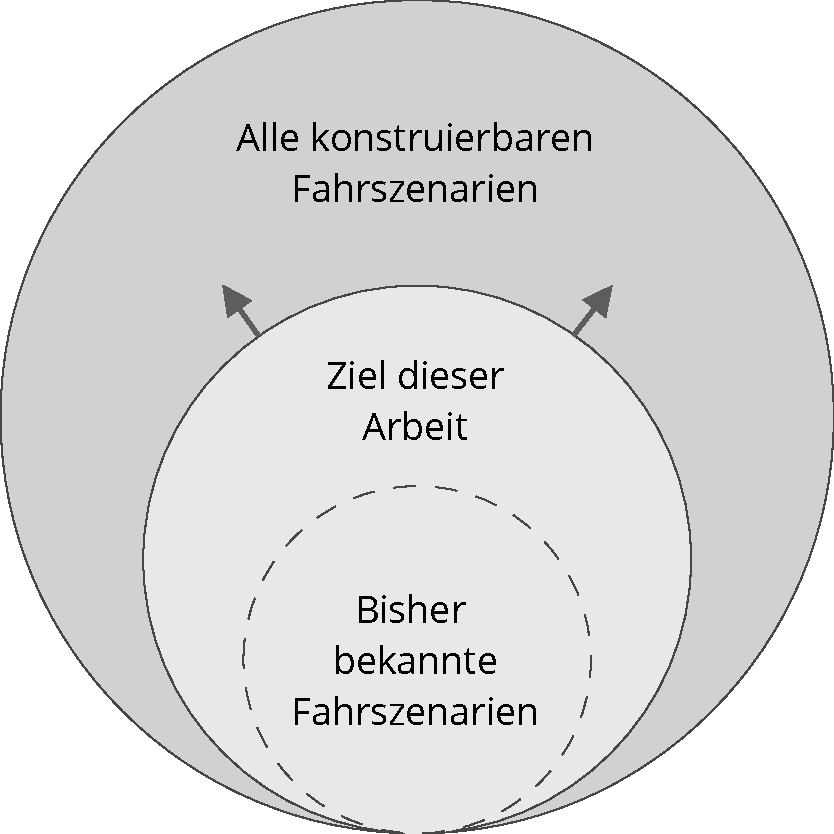
\includegraphics[scale=0.5]{teilmenge_fahrszenarien.pdf}
\caption{Beziehung zwischen bekannten und unbekannten Fahrszenarien}
\label{fig_teilmenge_fahrszenarien}
\end{figure}

In dieser Arbeit soll ein Proof-of-Concept für diese Methodik entwickelt werden. Dafür wird im folgenden Abschnitt \ref{konzept_struktur} das Konzept im Detail und die Vorgehensweise vorgestellt. Anschließend wird in Abschnitt \ref{konzept_methodik} die Methodik erklärt mit welcher dieses Konzept umgesetzt werden soll.

- funktionale Dekomposition

% ===========================
\section{Struktur}
\label{konzept_struktur}
% ===========================

- Definition von Fahrszenarien
- Simulation von Fahrten mit diesen Szenarien
- Extraktion und Labeling der Fahrszenarien
- Extraktion von Reale Fahrszenarien
- Training NN mit synthetischen und realen
- Evaluation mit realen Fahrszenarien

Im ersten Schritt der Umsetzung werden bestimmte Fahrszenarien ausgewählt und, wie in Abschnitt \ref{grundlagen_fahren_szenarien} erläutert, definiert. In dieser Arbeit werden Szenarien auf der Ebene der \textit{logischen Szenarien} definiert. Für das Training eines Klassifikators werden im nächsten Schritt synthetische und reale Daten benötigt.

Für die Generierung von synthetischen Daten 



Gleichzeitig bleibt der Aufwand für das Labeling der Daten überschaubar, weil die synthetischen Daten automatisiert gelabelt werden können und die realen Daten nur einen geringen Anteil ausmachen sollen.

% ===========================
\section{Methodik}
\label{konzept_methodik}
% ===========================

Lorem ipsum dolor sit amet, consetetur sadipscing elitr, sed diam nonumy eirmod tempor invidunt ut labore et dolore magna aliquyam erat, sed diam voluptua. At vero eos et accusam et justo duo dolores et ea rebum. Stet clita kasd gubergren, no sea takimata sanctus est Lorem ipsum dolor sit amet.  






